\chapter{Polynomial Evaluation}
\section{Introduction}
We will consider the following situation: $R$ is a commutative ring  as always and $f\in R[x]$ where $\deg(f)=d$. We also have $k$ points $u_0,\dots, u_{k-1}\in R$. Now we want to discuss here the fast algorithms of finding out $(f(u_0),\dots, f(u_{k-1}))$. So we basically want the evaluation map 
\begin{align*}
		\varphi: R[x]/\la m\ra & \to R^n\\ f & \to (f(u_0),\dots, f(u_{k-1}))
\end{align*}which is a ring homomorphism. If $R$ is a field then $R[x]$ is a vector space over $R$ and the $\phi$ is an isomorphism. Formally we want to solve the following two problems with fast algorithms:
\pr[singleeva]{Single Point evaluation}{Given $f\in R[x]$ with $\deg(f)=d$ and $\alpha\in R$ compute $f(\alpha)$}
\pr[multieva]{Multi-Point evaluation}{Given $f\in R[x]$ with $\deg(f)=d$ and $u_o,\dots, u_{n-1}\in R$ compute $f(u_0),\dots, f(u_{n-1})$}
\pagebreak

\section{Single Point Evaluation}
\subsection{Horner's Method}
\begin{Theorem}{Horner's Method}{horner}
	Given a polynomial $f(x)=\sum\limits_{i=0}^d a_ix^i$ where $a_i\in R$ for all $i\in [n]$ and a point $\alpha\in R$ using only $O(d)$ many additions and multiplications.
\end{Theorem}


\begin{myproof}Consider the following algorithm:
	
	\algo[horner]{$p(x)=a_0+x(a_1+x(a_2+(x(\cdots + x(a_n)\cdots))))$}{Horner's Method}
	
	Clearly we are using only $d$ many additions and $d$ many multiplications. So overall we need $2d=O(d)$ ring operations to evaluate the polynomial. The following lower bound results we obtain.
\end{myproof}
This is the minimal number of additions and multiplications for any algorithm to evaluate a polynomial.
\thm{\cite{horneraddlowerbound}}{Any algorithm to evaluate an arbitrary degree $d$ polynomial $f\in R[x]$ at any point $\alpha\in R$ must use at least $n$ additions}

\thm{\cite{hornermultlowerbound}}{Any algorithm to evaluate an arbitrary degree $d$ polynomial $f\in R[x]$ at any point $\alpha\in R$ without initial conditioning of coefficients has at least $n$ multiplications  and at least $n$ additions.}
\thm{\cite{hornermultlowerbound},\cite{motzkin}}{Any degree $d$ real polynomial can be evaluated using $\lt\lfloor \dfrac{d}2\rt\rfloor + 2$ multiplications and $d$ additions.}

\section{Fast Multi-point Evaluation}

A trivial algorithm for using $O(d^2)$ ring operations is to apply \hyperref[th:horner]{Horner's Method} for each point and since it takes $O(d)$ operations for each point we can find the evaluations at all $d$ points in $O(d^2)$ many ring operations. But we want to get close to linear operations. Since Horner's rules uses lowest number of ring operations doesn't mean for $d$ points $O(d^2)$ is lowest. There is an fast algorithm to evaluate the polynomial at all $d$ points using $O(M(d)\log d)$ operations.

\begin{center}
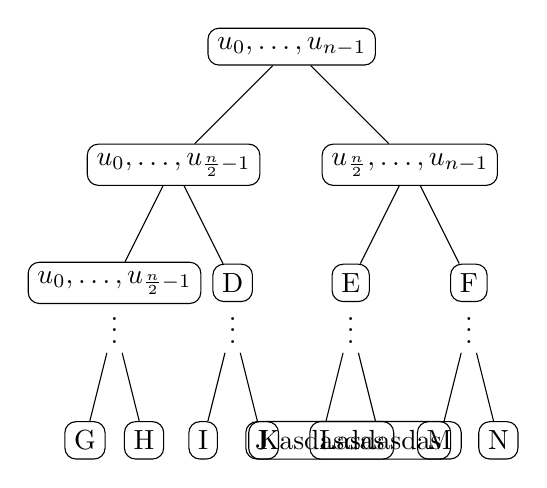
\begin{tikzpicture}[
	node distance=1.5cm,
	every node/.style={draw, rounded corners, rectangle, align=center},
	level/.style={sibling distance=3cm/2^(#1-1)},
	dot/.style={fill=black, circle, minimum size=0.1cm, inner sep=0pt}
	]

		
		% Nodes
		\node {$u_0,\dots, u_{n-1}$}
		child { node {$u_0,\dots, u_{\frac{n}2-1}$}
			child { node {$u_0,\dots, u_{\frac{n}2-1}$} 
				node[draw=none, yshift=-0.5cm] {$\vdots$}
				child { node {G} }
				child { node {H} }
			}
			child { node {D}
				node[draw=none, yshift=-0.5cm] {$\vdots$}
				child { node {I} }
				child { node {J} }
			}
		}
		child { node {$u_{\frac{n}{2}},\dots, u_{{n}-1}$}
			child { node {E}
				node[draw=none, yshift=-0.5cm] {$\vdots$}
				child { node {Kasdasdas} }
				child { node {Lasdasdas} }
			}
			child { node {F}
				node[draw=none, yshift=-0.5cm] {$\vdots$}
				child { node {M} }
				child { node {N} }
			}
		};
	\end{tikzpicture}
\end{center}